



\section{Social Interaction with Social World Model}
\label{sec:building_swm}
Building on the effectiveness of \protocolname as a structured social world representation,
We propose a SWM algorithm with \protocolname, enabling LLMs to model and predict social dynamics in first-person interactive settings, similar to how humans infer others’ mental states \citep{frith2006neural, Forrester1971}.






\paragraph{Foresee and Act with Social World Model}
We propose \texttt{Foresee and Act}, a simple inference-time algorithm that enables agents to simulate the consequences of their actions before committing to them. As shown in Figure~\ref{fig:swm-agent}, the agent first samples a candidate action at each timestep. Then, with the SWM, it simulates how the social state would evolve, including how other agents might interpret the action and how the environment might respond. 
In our implementation, one LLM predicts the next social world state, and another LLM generates agent's action and refines it based on the simulated outcome. 
\begin{figure*}[ht]
    \centering
    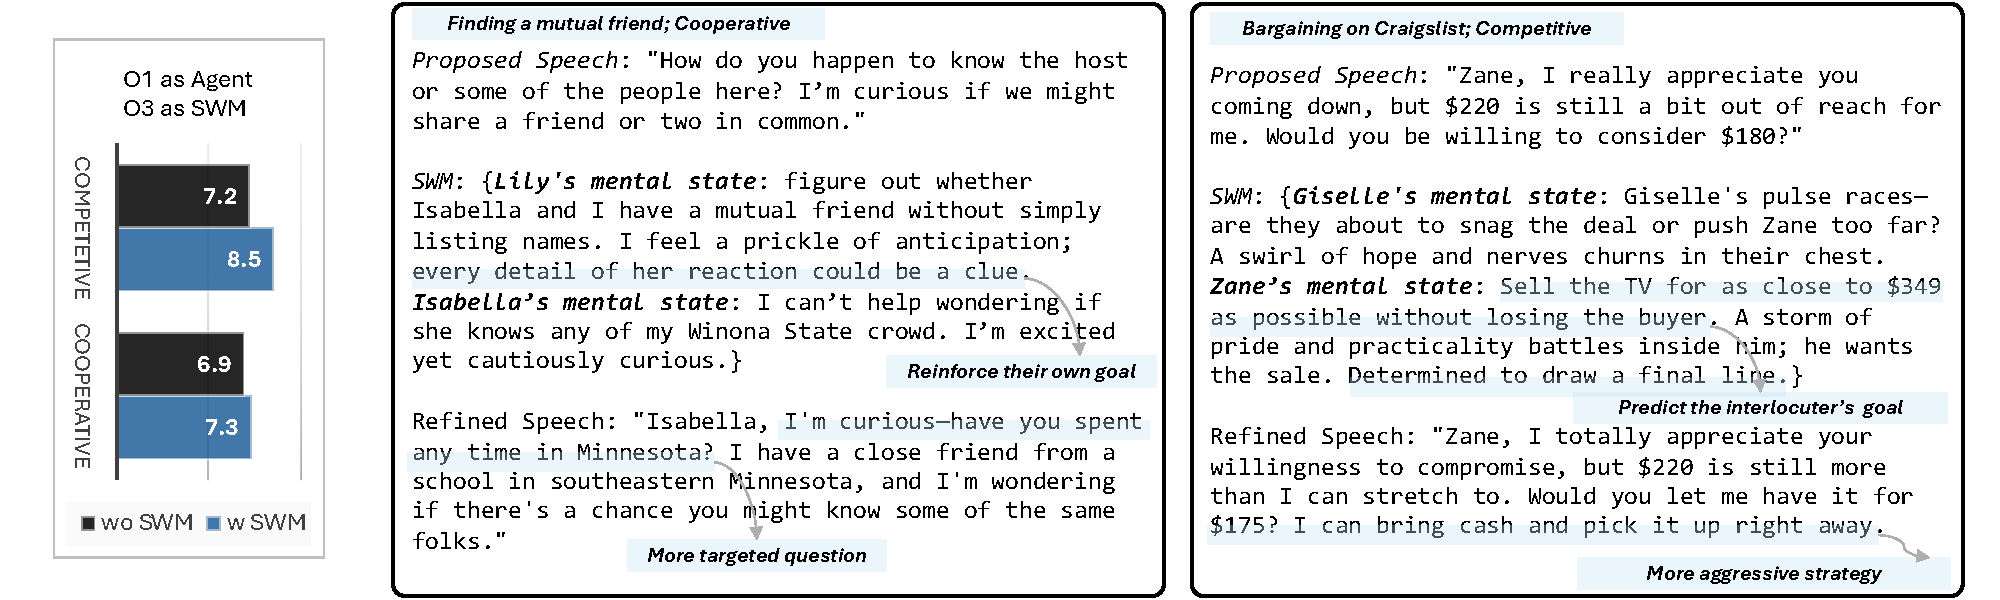
\includegraphics[width=\textwidth]{figs/swm-agent-example-fig5.pdf}
    \caption{SWM improves agent decision-making in both cooperative and competitive scenarios. The left most panel shows the overall performance of the agent (\texttt{o1}) with or without a SWM.}
    \label{fig:swm-agent-example}
\end{figure*}
\subsection{Experiment Setup}
\label{subsec:sotopia_experiment_setup}
We use SOTOPIA \citep{zhou2024sotopia}, the standard benchmark for goal-driven interactive social reasoning.
We use the SOTOPIA-hard evaluation set, which features more challenging social scenarios.
Each task features two characters with private social goals interacting within a given scenario. During each episode, two agents, a partner and a target of evaluation, play the characters to pursue their hidden goals.
In the end, a goal completion score (0-10) is assigned to each agent based on their performance.
We evaluate each model on 100 simulations from the SOTOPIA-hard set %
with \texttt{GPT-4o} as the fixed partner agent and show results for \texttt{o3}, \texttt{o1}, \texttt{GPT-4.1}, and Llama 4 Maverick Instruct (\texttt{Llama-4}) to serve as either the agent, or the social world model, using a one-step SWM rollout to assess the effect of SWM.



\subsection{Social World Modeling Results}
Figure~\ref{fig:model_performance_comparison} shows that integrating an \protocolname-powered social world model consistently boosts agent performance in social interactions. %
Interestingly, stronger social agents do not always yield better social world models, for instance, \texttt{GPT-4.1} outperforms Llama 4 Maverick as an agent (6.01 vs. 4.52), yet their SWM performance is nearly identical (6.34 vs. 6.36).
This supports the view in \S\ref{sec:omniscient_social_reasoning} that social reasoning involves two parts, and strength in constructing social representations doesn't imply strength in reasoning over them and acting correctly.
Moreover, even when the SWM offers useful information (e.g., \texttt{o1}), the paired agent's performance can still drop (e.g., with Llama 4 Maverick), highlighting a key challenge: to benefit from social world modeling, agents must be able to effectively incorporate the modeled information into their decision-making.
Additional analysis of model pairings and baseline performance can be found in Appendix~\ref{app:sotopia_additional} (Figures~\ref{fig:sotopia_heatmap} and~\ref{fig:sotopia_vanilla}).


\paragraph{Analysis on the impact of SWM}
To better understand the role of social world models in multi-agent interactions, we evaluate SWM in both cooperative and competitive settings.
In the cooperative setting, agents pursue a shared social goal (e.g., Ben and Alice want to identify mutual friends, and they need to chat with each other to find the mutual friends effectively), while in the competitive setting, agents have conflicting goals (e.g., In the barter scenario, Ben and Alice want to trade a TV for a laptop, but they need to negotiate with each other to find a mutually agreeable price).
We run 100 simulations per setting using \texttt{o1} as the agent and \texttt{o3} as the SWM. As shown in Figure~\ref{fig:swm-agent-example}, SWM improves performance in both cases, with larger gains in competitive cases. 
In these cases, the agent can better anticipate and strategically respond to the opponent's moves.
Regradless of the setting, tracking and predicting the intentions and beliefs of other agents is important for successful social interactions, which is the key function of a social world model.













